% Options for packages loaded elsewhere
\PassOptionsToPackage{unicode}{hyperref}
\PassOptionsToPackage{hyphens}{url}
%
\documentclass[
  a4paperpaper,
  twocolumn]{article}
\usepackage{lmodern}
\usepackage{amssymb,amsmath}
\usepackage{ifxetex,ifluatex}
\ifnum 0\ifxetex 1\fi\ifluatex 1\fi=0 % if pdftex
  \usepackage[T1]{fontenc}
  \usepackage[utf8]{inputenc}
  \usepackage{textcomp} % provide euro and other symbols
\else % if luatex or xetex
  \usepackage{unicode-math}
  \defaultfontfeatures{Scale=MatchLowercase}
  \defaultfontfeatures[\rmfamily]{Ligatures=TeX,Scale=1}
\fi
% Use upquote if available, for straight quotes in verbatim environments
\IfFileExists{upquote.sty}{\usepackage{upquote}}{}
\IfFileExists{microtype.sty}{% use microtype if available
  \usepackage[]{microtype}
  \UseMicrotypeSet[protrusion]{basicmath} % disable protrusion for tt fonts
}{}
\makeatletter
\@ifundefined{KOMAClassName}{% if non-KOMA class
  \IfFileExists{parskip.sty}{%
    \usepackage{parskip}
  }{% else
    \setlength{\parindent}{0pt}
    \setlength{\parskip}{6pt plus 2pt minus 1pt}}
}{% if KOMA class
  \KOMAoptions{parskip=half}}
\makeatother
\usepackage{xcolor}
\IfFileExists{xurl.sty}{\usepackage{xurl}}{} % add URL line breaks if available
\IfFileExists{bookmark.sty}{\usepackage{bookmark}}{\usepackage{hyperref}}
\hypersetup{
  pdftitle={Pizza - A Carbohydrate Based Substrate For Tomato Delivery},
  pdfauthor={Maxwell Ogden, Pizza Enthusiasts Institute},
  hidelinks,
  pdfcreator={LaTeX via pandoc}}
\urlstyle{same} % disable monospaced font for URLs
\usepackage{graphicx,grffile}
\makeatletter
\def\maxwidth{\ifdim\Gin@nat@width>\linewidth\linewidth\else\Gin@nat@width\fi}
\def\maxheight{\ifdim\Gin@nat@height>\textheight\textheight\else\Gin@nat@height\fi}
\makeatother
% Scale images if necessary, so that they will not overflow the page
% margins by default, and it is still possible to overwrite the defaults
% using explicit options in \includegraphics[width, height, ...]{}
\setkeys{Gin}{width=\maxwidth,height=\maxheight,keepaspectratio}
% Set default figure placement to htbp
\makeatletter
\def\fps@figure{htbp}
\makeatother
\setlength{\emergencystretch}{3em} % prevent overfull lines
\providecommand{\tightlist}{%
  \setlength{\itemsep}{0pt}\setlength{\parskip}{0pt}}
\setcounter{secnumdepth}{-\maxdimen} % remove section numbering

\title{Pizza - A Carbohydrate Based Substrate For Tomato Delivery}
\author{Maxwell Ogden, Pizza Enthusiasts Institute}
\date{May 2017}

\begin{document}
\maketitle

\hypertarget{abstract}{%
\section{Abstract}\label{abstract}}

Pizza (Pizza et al. (2000)) is an understudied yet widely utilized
implement for delivering in-vivo \emph{Solanum lycopersicum} based
liquid mediums in a variety of next-generation mastications studies.
Here we describe a de novo approach for large scale \emph{T. aestivum}
assemblies based on protein folding that drastically reduces the
generation time of the mutation rate.

\hypertarget{diagram}{%
\section{Diagram}\label{diagram}}

\begin{figure}
\centering
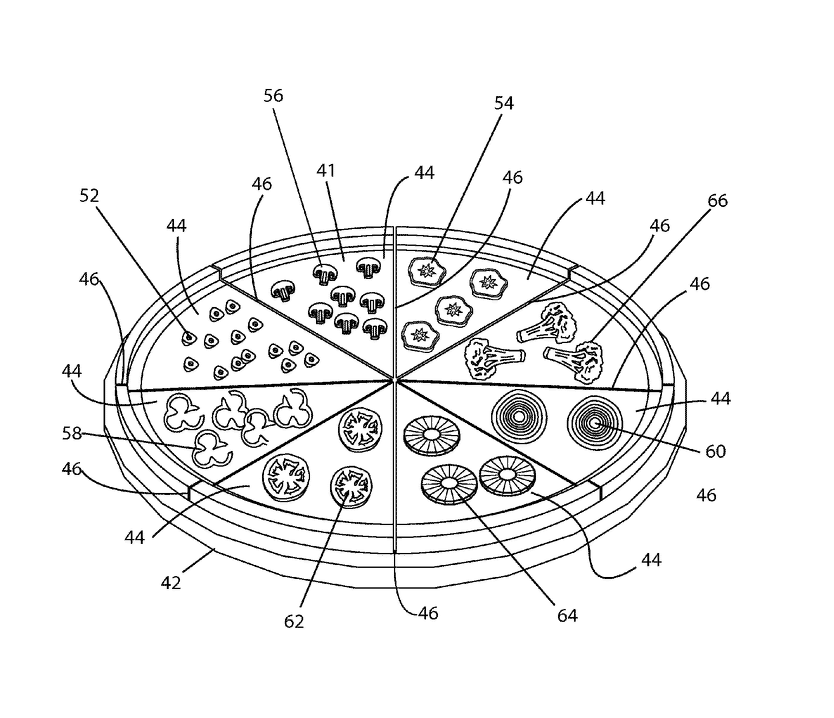
\includegraphics{https://gist.github.com/maxogden/97190db73ac19fc6c1d9beee1a6e4fc8/raw/adaaa9b5c19460d3be42021ef0c1b8e11a8d38fe/pizza.png}
\caption{It's Pizza}
\end{figure}

\hypertarget{algorithm}{%
\section{Algorithm}\label{algorithm}}

\[f(x)=pizza^2\]

\hypertarget{references}{%
\section*{References}\label{references}}
\addcontentsline{toc}{section}{References}

\hypertarget{refs}{}
\leavevmode\hypertarget{ref-pizza2000identification}{}%
Pizza, Mariagrazia, Vincenzo Scarlato, Vega Masignani, Marzia Monica
Giuliani, Beatrice Arico, Maurizio Comanducci, Gary T Jennings, et al.
2000. ``Identification of Vaccine Candidates Against Serogroup B
Meningococcus by Whole-Genome Sequencing.'' \emph{Science} 287 (5459):
1816--20.

\end{document}
